\chapter{电脑以及电脑的组成}
\label{computer-and-its-components}

\begin{intro}
  在这一部分,我们将对「电脑」这种神奇的黑箱做一个简要的、整体的介绍。看完这一部分,你将可以找到这些问题的答案:

  \begin{itemize}
    \item 什么是「CPU」?他们说的「i5」「i7」都是什么?「双核」「四核」又是什么?
    \item 为什么说「内存和硬盘不一样」?为什么手机上我们都喊「内存」?电脑特别卡,到底是内存不够还是硬盘不够?
    \item 我想玩游戏,选购电脑时应该关注什么方面?
    \item 什么是「Windows」?那「Windows 10」又是什么?为什么那些用苹果笔记本的同学电脑界面看起来和我不一样?
  \end{itemize}
\end{intro}

电脑是由电路部分的硬件和电路之上的软件部分组成的。在大多数使用电脑的时候,我们都只与屏幕上的画面、窗口、文件打交道,但其实我们在使用过程中的许多问题都要牵涉到电脑的基本硬件设施。在本章,我们不妨先来看看电脑那内部几乎不为所见的「硬」的一面,之后再去看看为人所见却不甚了解的「软」的一面。

\section{电脑内部的硬件} 

这一节我们来介绍一台电脑内部的那些关键硬件。也许你并没有亲眼见过这些芯片和设备长什么样,但通过这一节的介绍,你应该能对它们有一个基本的了解。

\subsection{想象一个场景……}

我们先不谈硬件那些抽象的东西,我们假设这样一个场景:老师收了一个班的一摞作业,现在需要批改这些作业。

\begin{figure}[htb!]
  \centering
  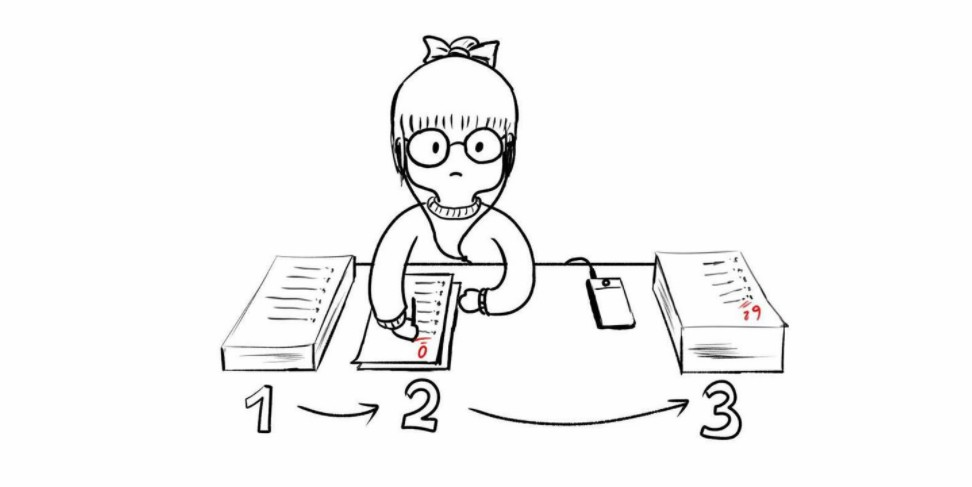
\includegraphics[width=7cm]{assets/Teacher_and_homework.jpg}
  \caption{老师和她需要批改的作业}
  \label{teacher-and-homework}
\end{figure}

就如图 \ref{teacher-and-homework} 所绘的那样,老师批改作业的过程,可以简单地分解为下面这样几个步骤:

\begin{enumerate}
  \item 老师将这一摞作业堆在办公桌的一边,腾出办公桌的中央和另一边。
  \item 现在,老师取下这一摞作业中的一小叠,放在办公桌中央,开始伏案批改。
  \item 老师批改完了这一小叠作业,然后将它们放在办公桌的另一边,摞成新的一沓。
  \item 重复步骤 2 和步骤 3,最终老师完成了全部作业的批改,这时批改完的作业全部在办公桌的另一边。
\end{enumerate}

我们会借助这个例子来更好地理解电脑硬件上的各个结构。

\subsection{处理器 / CPU}

中央处理器,简称「处理器」,英文简写「CPU」,是电脑内部最重要的一枚芯片,可以想象成是电脑的「大脑」。在上面的例子中,「老师」就相当于电脑中的处理器:「老师」的作用是对「作业」进行批改,从而完成教学任务;处理器的作用是进行各种的运算,从而实现电脑不同的功能。

你一定注意到过,电脑会发热——热到需要用一个风扇给它降温,这热量中有很大一部分就是处理器发出来的。如果你有关注过时事和新闻,中美贸易战中的「芯片」战,其中关键的一环就是处理器芯片。下图中,左为常见的台式电脑的 CPU 芯片,右为常见的笔记本电脑的 CPU 芯片。

\begin{figure}[H]
  \centering
  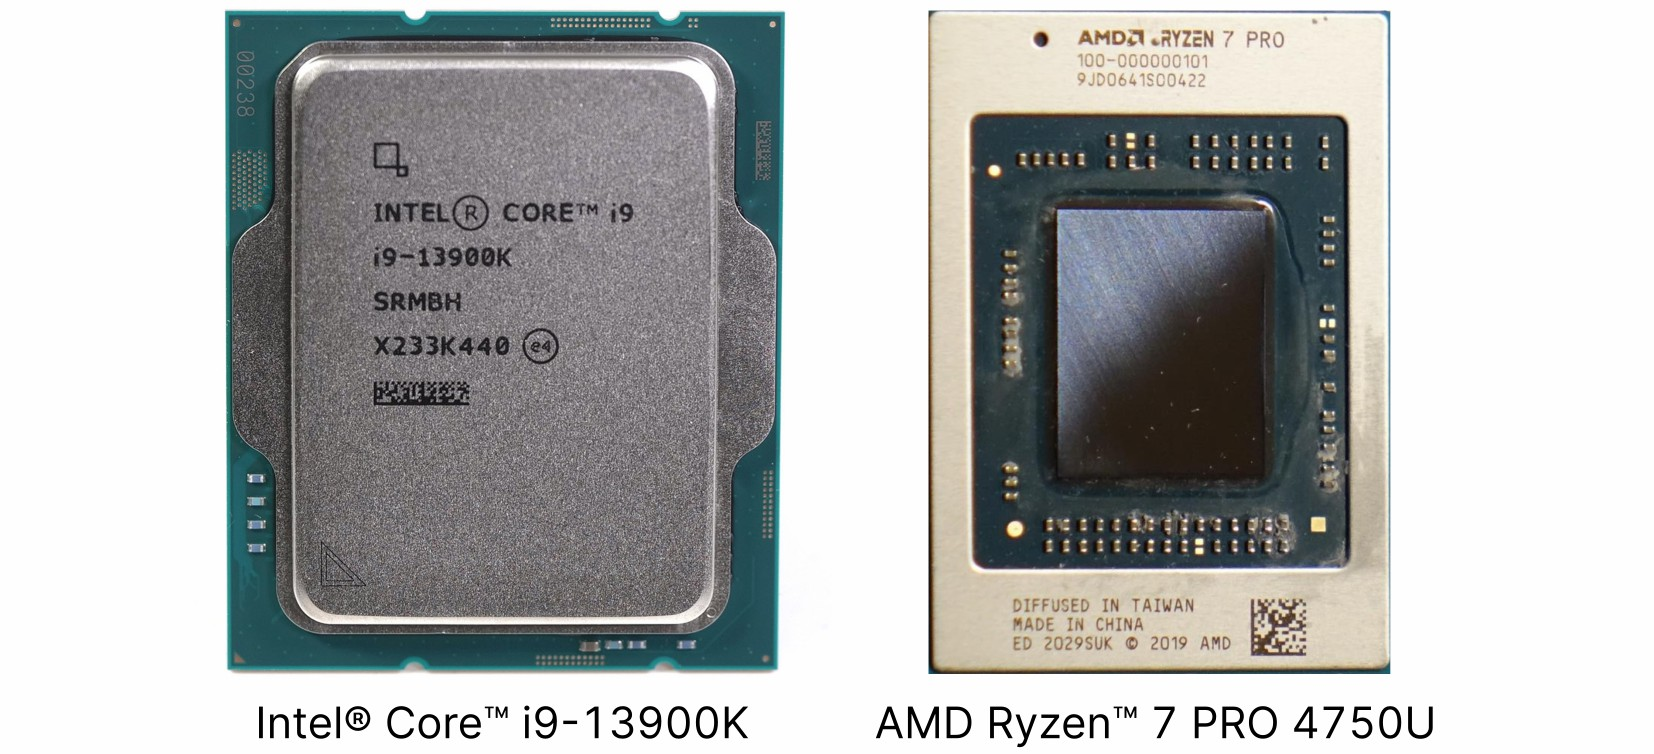
\includegraphics[width=10cm]{assets/CPUs.jpg}
  \caption{常见的台式机和笔记本电脑的处理器芯片。}
  \label{cpus}
\end{figure}

处理器是电脑工作的核心芯片,\regcolor{因此,处理器的性能就很大程度上决定了电脑的性能,决定了我们使用这台电脑流不流畅、玩游戏卡不卡、工作效率高不高}。在今天,全世界电脑芯片基本上是由两家美国公司设计制造\footnote{事实上,芯片的「设计」和「制造」两件事是不一样的,就像能设计出房屋的建筑师不一定会到工地上去砌墙。英特尔能够自行完成从设计到制造整条流水线,而 AMD 只能完成设计,它的处理器是由专门负责制造芯片的厂商(例如台积电)生产的。}的,其中一家叫做「英特尔」(Intel),另一家叫做「AMD」。

\begin{itemize}
  \item 英特尔公司现在主要的 CPU 产品线称作「酷睿」(Core),而「酷睿」系列又分成了 4 个档次——「i3」「i5」「i7」和「i9」。
    如果你现在在用笔记本电脑,不妨瞄一眼键盘下方是否有如图 \ref{stickers-of-intel} 那样一个蓝色(也有可能是灰色,这里没有列出)的贴纸。
    \begin{figure}[htb!]
      \centering
      \begin{minipage}{8cm}
        \centering
        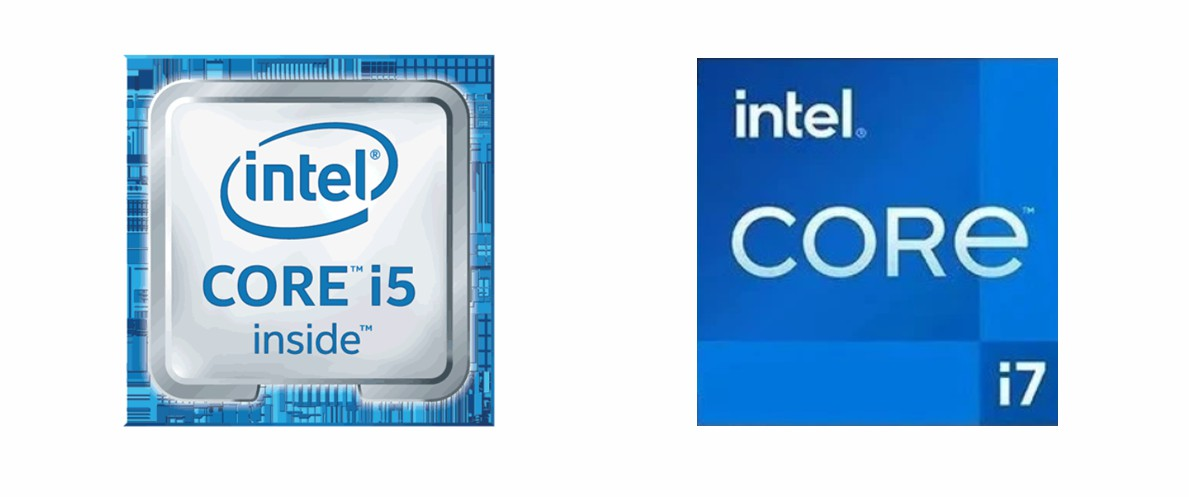
\includegraphics[width=6cm]{assets/Stickers_Intel.jpg}
        \caption{英特尔的贴纸}
        \label{stickers-of-intel}
      \end{minipage}
      \qquad
      \begin{minipage}{5cm}
        \centering
        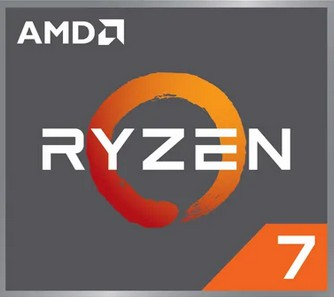
\includegraphics[width=2cm]{assets/Sticker_AMD.jpg}
        \caption{AMD 的贴纸}
        \label{sticker-of-amd}
      \end{minipage}
    \end{figure}
  \item AMD 公司现在主要的 CPU 产品线称作「锐龙」(Ryzen),而「锐龙」系列也分成了 3 个档次——「R5」「R7」和「R9」\footnote{其实还有 R3,但是很少在消费市场见到。}。
    如果你现在用笔记本电脑,不妨瞄一眼键盘下方是否有如图 \ref{sticker-of-amd} 那样一个红色的贴纸。
\end{itemize}

我们常常说一台电脑是「双核」「四核」的,这里的「双核」「四核」也是处理器中的概念。这些处理器在一片芯片放了多个「核心」,相当于一个个协同起来的独立的小处理器。例如「双核」处理器,意味着在一枚处理器芯片上集成了两个核心,相当于两个大脑协同工作,当我们需要用电脑同时做很多事情的时候就有所裨益。同理,「四核」「八核」就是在一个芯片上集成了四个甚至是八个核心。

需要强调的是,\regcolor{并不是说核心数越多的处理器性能一定越好},更\regcolor{不是说 i7 处理器就一定比 i5 更好},也\regcolor{不是说英特尔的处理器就要比 AMD 好}。我们应该这样辩证地理解这些概念:每个品牌都有自己的不同系列,有的系列高端,有的系列低端;每个系列也都有自己的不同型号,有的型号性能强,有的型号性能弱。CPU 的性能并不与某一个因素呈线性的关系,而是多个因素综合的结果。

\subsection{内存 / RAM}

紧接着,我们介绍能直接与处理器交流的部件——内存,英文简写「RAM」。上一小节提到,处理器相当于大脑,但与大脑不同的是,处理器只能\regcolor{处理}数据,而这些待处理的数据,需要依赖外部的元件来临时存储。内存就是用来临时存储数据的。

内存本质也是一组芯片。生产内存这种芯片和生产处理器那种芯片所用的工艺有一些不同,目前生产内存这种芯片的厂商集中在韩国和中国台湾。一般这些芯片被排在条形的电路板上,这样的整体叫做「内存条」。下图中,上方的内存条是台式电脑使用的,下方的内存条是笔记本电脑使用的。

\begin{figure}[H]
  \centering
  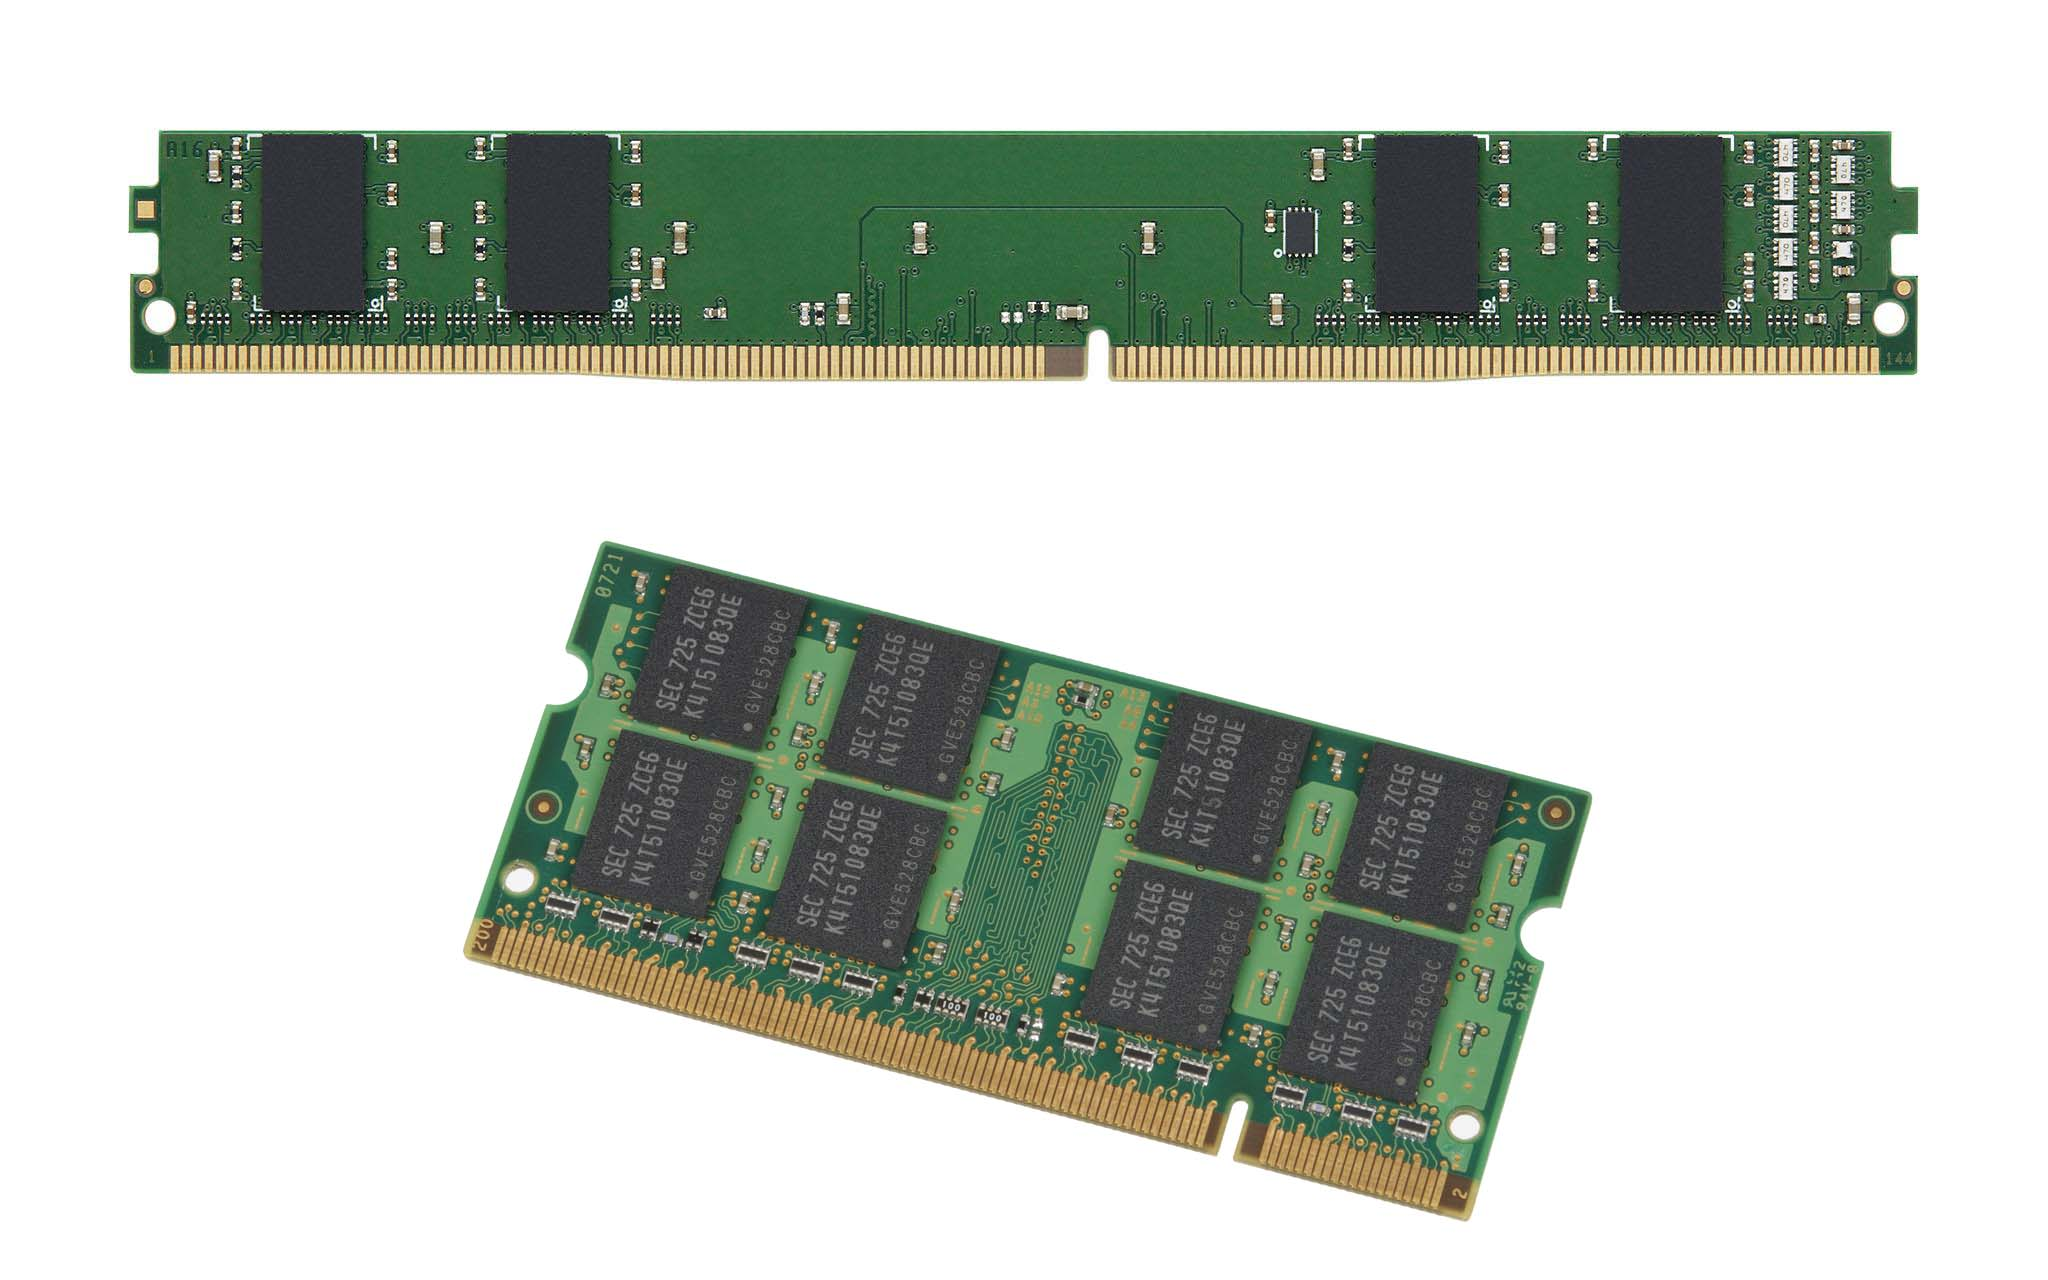
\includegraphics[width=8cm]{assets/RAMs.jpg}
  \caption{常见的内存条}
  \label{rams}
\end{figure}

前文说,内存直接与处理器进行数据交流。与处理器那极快的运算速度相匹配,内存的读取与写入速度也是极快的。但\regcolor{内存有一个特点——断电即丢失数据}。也就是说,当你电脑关机,内存中的数据便不复存在,又回到白纸一块。如果你想在内存里长久存放数据,那唯一的做法就是一直通电,多浪费电啊是吧。

回到前面老师批改作业的场景。办公桌的中央区域可以理解为「内存」:老师将作业放在办公桌中央批改,是因为这里改起来最方便;处理器将数据放在内存中处理,是因为这里读取和写入速度最快。办公桌中央不能总是放着东西,不然会弄乱、弄丢;内存中的数据一旦断电就会消失,因此总是临时的。

在 21 世纪初技术不是很发达的时候,内存的容量也不是很大,有 512 MB 已经不得了了。但随着时间的流逝,现如今大容量内存已经司空见惯。要想让现今的普通电脑基本流畅运行,内存容量应当至少有 4 GB。当然这东西倒是多多益善,就像更大的桌子能摆更多东西一样,\regcolor{更多的内存意味着更多的空间来让处理器存放数据,也就意味着电脑能同时处理更多的任务,基本意味着电脑更加流畅。}据我们的经验,流畅运行诸如 AutoCAD、Photoshop 之类的专业软件至少需要 8 GB 的内存。整体来说,在目前(2023 年),16 GB 的内存对于绝大多数人都已经够用了。

\begin{note}
  对应到手机中,内存有时会被手机厂商称为「运行内存」,不过我们不推荐如此称呼。
\end{note}

\subsection{硬盘}

内存是用来临时存储数据的,而硬盘则是用来长久保存数据的。与内存相比,硬盘的读写速度要慢得多,但存在硬盘中的数据不会因为断电而轻易消失,因此,\regcolor{硬盘是数据的最初的起点和最终的归宿}:处理器在一开始,从硬盘中取出数据放入内存,在内存中处理数据,处理完成之后,再将新的数据放回硬盘。

在前面老师批改作业的场景当中,办公桌两侧堆作业的地方可以理解为「硬盘」:大量的作业被堆在那里,整齐摆放,不会弄散、弄丢,但老师总是要把作业取到趁手的地方(办公桌中央)来批改;大量的数据被存在硬盘里,不会因为断电就丢失,但处理器总是要把数据放在快速的地方(内存)来处理。

简单来说,硬盘现在分为两种,一种叫「机械硬盘」(英文简称「HDD」)如下图左侧所示,一种叫「固态硬盘」(英文简称「SSD」)如下图右侧所示。
前者容量大、价格低、速度更慢,后者容量小、价格高、速度较快(但远远没有内存那么快)。
前者是利用电磁原理存储数据,后者是芯片存储数据,但这种芯片和内存的那种又不一样——内存那种断电数据就消失了,固态硬盘的芯片断电还能保持数据。
但要注意,如果硬盘许久不用(不给它通电),那里面的数据也会慢慢消失,固态硬盘大约是 3 至 5 年,而机械硬盘最多 20 年,所以没事的时候记得把存了东西的硬盘拿出来让它动一动。

\begin{figure}[H]
  \centering
  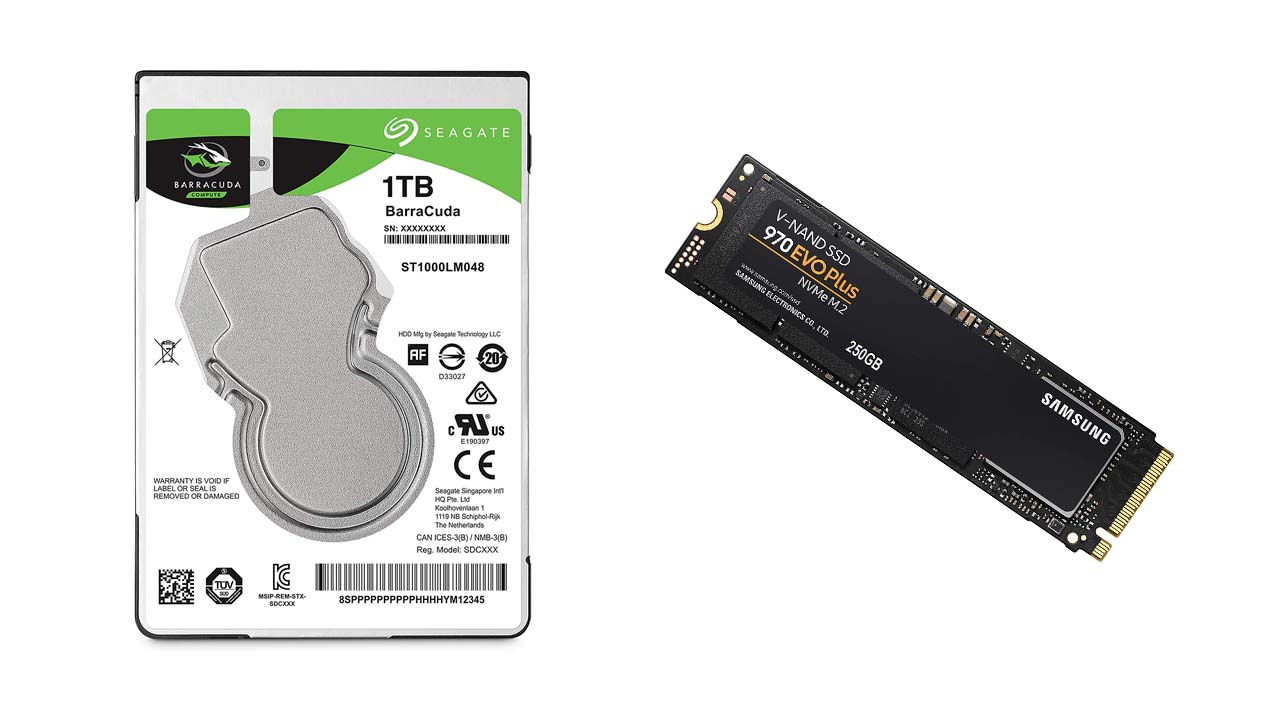
\includegraphics[width=8cm]{assets/Disks.jpg}
  \caption{常见的硬盘}
  \label{disks}
\end{figure}

在今天(2023 年),标称容量 1 TB 的固态硬盘大约 500 元,机械硬盘大约 300 元;标称容量 2 TB 的固态硬盘大约 900 元,机械硬盘大约 450 元。
今天的中档次电脑常见的组合是用一块小容量(比如 512 GB)的固态硬盘,搭配一块大容量(比如 1 TB)的机械硬盘来实现各自功能的互补。
稍微高档次一点的电脑,则会选用一整块更大容量(比如 1 TB 甚至 2 TB)的固态硬盘而不再使用机械硬盘。

打开桌面上的【此电脑】,你看到的所谓「C 盘」「D 盘」,就是硬盘上的空间——一块硬盘的空间可以被划分成不同的「盘」(学名叫「分区」)来更好地利用。

\begin{figure}[H]
  \centering
  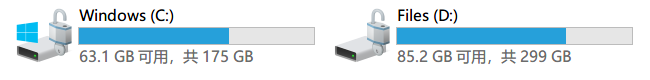
\includegraphics[width=10cm]{assets/Partition.png}
  \caption{一些分区}
  \label{partitions}
\end{figure}


\regcolor{硬盘对电脑使用体验的影响,主要是「打开软件的速度」,包括「开机的速度」}。这是很容易理解的,因为数据原先都是存在硬盘里的,处理器从硬盘里「拿」数据的速度就直接影响着软件启动或者说加载的时间。

\begin{note}
  手机中也有类似固态硬盘一样的芯片来存储数据,它有时候被手机厂商称为「存储内存」,但它\regcolor{完全不是}内存。这是为什么有人会弄混「内存」和「硬盘」的根源之一。大家常说的「手机内存不够」,指的往往是存储空间(可以理解为「手机的硬盘」)不够,而不是真正的「内存」不够。
\end{note}

\subsection{显卡 / GPU *}

对于喜欢玩游戏的同学来说,「显卡」是他们在选购电脑时会着重考虑的一个因素。

最开始,「显卡」就是电脑里面的一个独立的芯片,像内存那样有自己的独立的电路板并插接在主板上。
这个芯片的功能是专门进行画面的绘制和图像的处理,因而得名「显」卡。
所有显示在屏幕上的画面,都是由显卡进行「绘制」的。
因而\regcolor{显卡的性能主要是对游戏以及一些图形相关的工作(比如三维制图、视频剪辑)有较大影响}。

\begin{figure}[H]
  \centering
  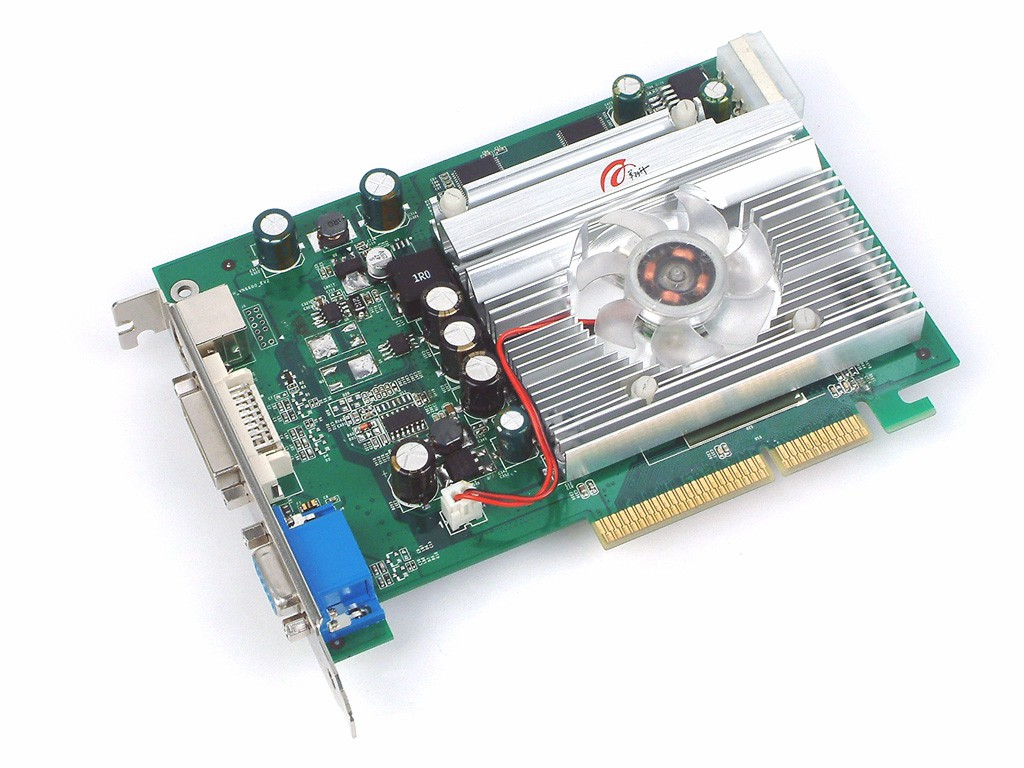
\includegraphics[width=8cm]{assets/Old_GPU.jpg}
  \caption{近 20 年前电脑上的显卡}
  \label{old-gpu}
\end{figure}

为什么上面那段要加上「最开始」三个字呢?因为随着半导体技术的发展,人们后来发现,显卡可以被「集成」到处理器\footnote{一开始,集成显卡并不是集成到处理器中的,而是集成在主板上的一个芯片之中(称为「北桥」),后来才集成到了处理器里面。}中,换言之,就像多核处理器把几个核心放在一个芯片上一样,显卡也可以和处理器放在一个芯片上。容易想到,这样集成到一起之后,显卡就不能做得很大了(受限于芯片整体的大小),也不能做得性能很强了(因为处理器核就在它边上,大家一起发热,一起分享能量),但可以缩小硬件的体积,也能降低功耗。因而,发展到今天,显卡在电脑中的形态有了以下两种:

\begin{itemize}
  \item \regcolor{集成显卡},英特尔称「核芯显卡」,AMD 称「APU」。显卡被安排在处理器的同一片芯片上,性能相对较差(但还是能应付大多数工作的,只是游戏、制图等特定工作就不太行了),功耗低,体积小。
  \item \regcolor{独立显卡},简称「独显」。显卡仍然是一片独立的芯片,有自己的供电和外围元件。这样的显卡性能比较强,但换来的是更高的功耗、更大的体积(游戏本为什么重)和更多的发热等。
\end{itemize}

\begin{figure}[H]
  \centering
  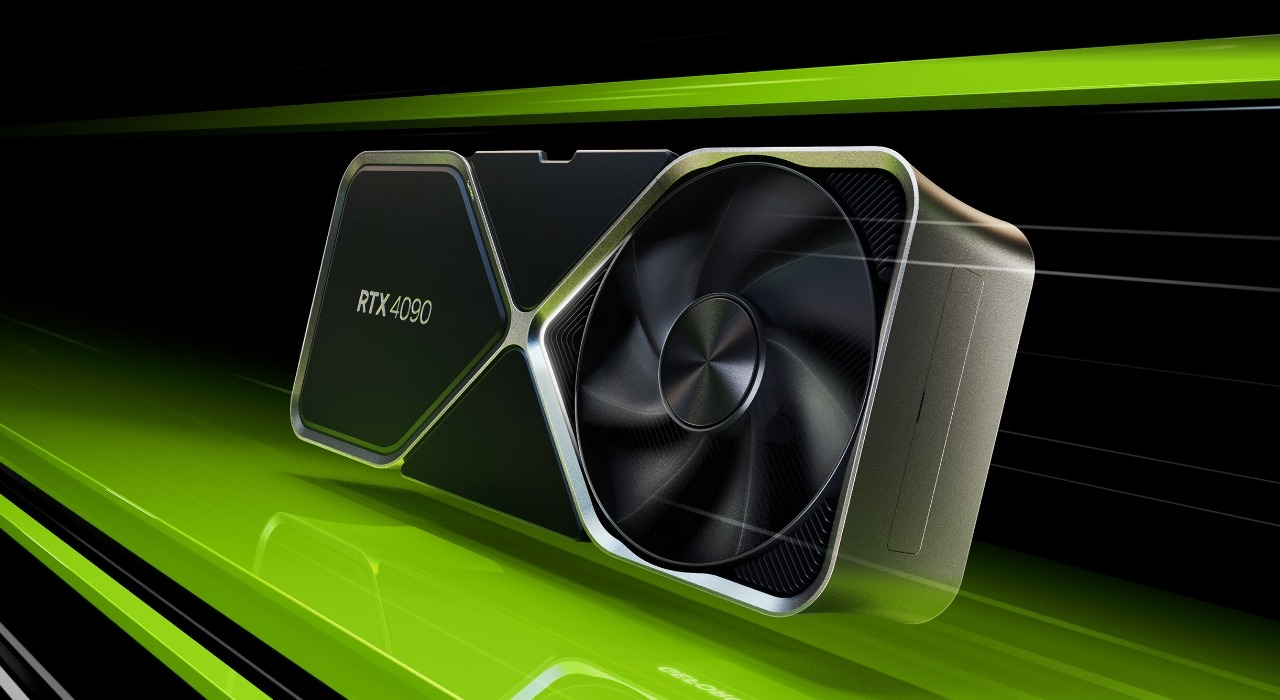
\includegraphics[width=6cm]{assets/RTX-4090.jpg}
  \caption{英伟达目前的顶级游戏显卡「RTX 4090」}
  \label{4090-gpu}
\end{figure}

今天,全世界生产\regcolor{独立显卡}的厂商主要有两家,一家叫「英伟达」(Nvidia),它生产的显卡俗称「N 卡」;另一家是前文提到过造处理器的「AMD」,它生产的显卡俗称「A 卡」。如果你有涉足过硬件交流圈,玩家所说的「RTX 3060」「GTX 1080 Ti」等都是英伟达显卡的型号,「RX 6800 XT」「RX 580」等都是 AMD 显卡的型号。上图是目前英伟达的顶级游戏显卡 RTX 4090。

\begin{note}
  是不是有人会问,那生产集成显卡的厂商有哪些呢?这个问题这里不回答,因为这不构成一个问题。
\end{note}


一般来说,对于笔记本,轻薄本都没有独立显卡而是使用集成显卡,游戏本都装配有独立显卡。这是由它们的使用场景和目标人群不同所决定的。

\section{与我们「打交道」的软件}

\subsection{软件与操作系统}

下面我们简单介绍「软件」和「操作系统」的概念。

由处理器、内存、硬盘以及各种各样的外围电子元件,共同构成了一台电脑的「硬件」部分。「硬件」就是电脑中电子电路的部分。而在「硬件」之上,硬件的具体工作任务是由「软件」来决定的。

我们用大家更熟悉的手机来做一个解释。\regcolor{手机上大家自己装的「QQ」「微信」「网易云音乐」,以及不是自己装的「电话」「短信」等 app 就属于「软件」}。「QQ」「微信」指导硬件去利用网络收发信息,利用屏幕展示数据,「网易云音乐」指导硬件去播放声音,同时在屏幕上展示评论,「电话」「短信」指导硬件利用无线电模块发送和接收信号……同样一部手机,硬件还是那个硬件,但能通过不同的软件行使不同的具体功能。

而在「QQ」「微信」「电话」等 app 之下,在纯粹的硬件之上,有\regcolor{一个更大,而且更「底层」的大软件,这个软件叫「操作系统」}。简单地说,操作系统「夹」在各个 app 和硬件之间,为 app 具体行使功能提供了一系列方便的「接口」。有了操作系统,网易云音乐的的开发者不再需要真正地去学习「怎么让喇叭发声」,而只需要学习「怎么告诉操作系统让喇叭发声」。「让喇叭发声」是一个带一些物理复杂知识的过程,但「告诉操作系统让喇叭发声」则相对简单得多。

\begin{figure}[H]
  \centering
  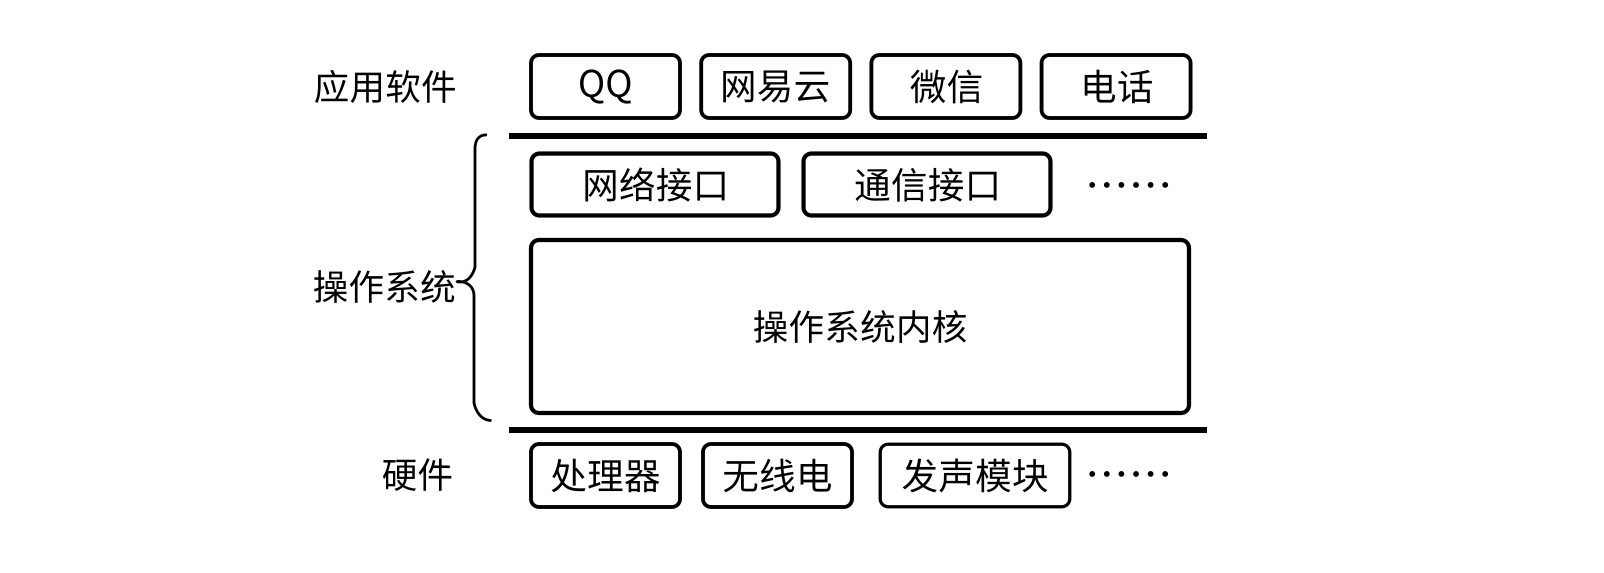
\includegraphics[width=13cm]{assets/Computer_Structure.png}
  \caption{App、操作系统和硬件的关系}
  \label{computer-structure}
\end{figure}

由于上层的软件(也就是 app)需要依赖操作系统来实现功能,而每个操作系统留给 app 的接口细节上也有所不同,因此,针对不同操作系统开发的软件是不能直接通用的。App 厂商一般会为不同的操作系统开发同一款 app,这样就能照顾到使用不同系统的用户。

今天主流的手机操作系统有「安卓」(Android)和「iOS」。
后者只能使用在 Apple 的硬件上,前者则被各个手机厂商使用\footnote{华为开发的「鸿蒙」(Harmony OS)由于以某种方式兼容安卓软件,在这里我们暂且作为前者对待。}。
而到了电脑上,「Windows」和「macOS」是最常见的两种操作系统,
后者只能使用在 Apple 的硬件上。
由于我们认为 macOS 的使用者不会依靠《Missing》来学习电脑知识,因而《Missing》中的所有操作都认定读者使用 Windows 系统。

下图为我们展示了 Windows 与 macOS 系统的典型界面。

\begin{figure}[htb!]
  \centering
  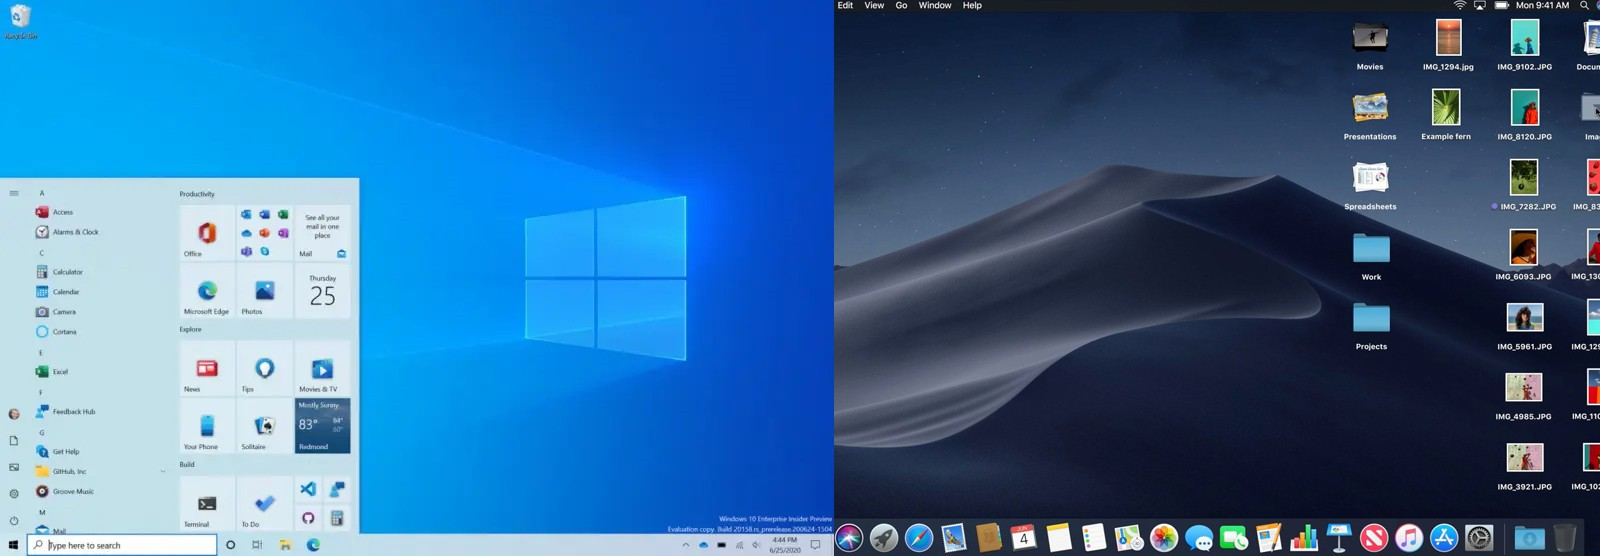
\includegraphics[width=11cm]{assets/Windows_and_macOS.jpg}
  \caption{Windows (左)和 macOS (右)}
  \label{win-and-mac}
\end{figure}

\subsection{Windows 操作系统}

我们的大多数人使用的都是 Windows 操作系统。所谓「Windows XP」「Windows 7」和「Windows 10」则是 Windows 操作系统的不同版本。

Windows 由美国的微软公司(Microsoft)所开发,诞生于 1985 年。到今天(2021 年),Windows 已经经历了数个大版本的更新\footnote{关于 Windows 的一点点更新历史,可以参见\nameref{recover-from-bsod}一章。}。目前最新的 Windows 版本是「Windows 11」(发布于 2021 年 10 月 5 日),我们大多数人使用的是「Windows 10」,还有一些稍旧的计算机在使用「Windows 7」。
更老的 Windows 版本,例如「Windows XP」,除去一些特定的老旧设备需要它们,日常已经鲜有使用。不同版本 Windows 系统之间会有操作细节、使用体验上的不同,不过往往最直观的不同是它们的「外观」。

Windows 可以使用在英特尔或者 AMD 处理器的电脑上——事实上,今天除了 Apple 以外几乎所有品牌的个人电脑都运行着 Windows 系统。通过右键桌面上的【此电脑】并点选【属性】,你可以看到自己电脑 Windows 系统的版本。

\begin{figure}[H]
  \centering
  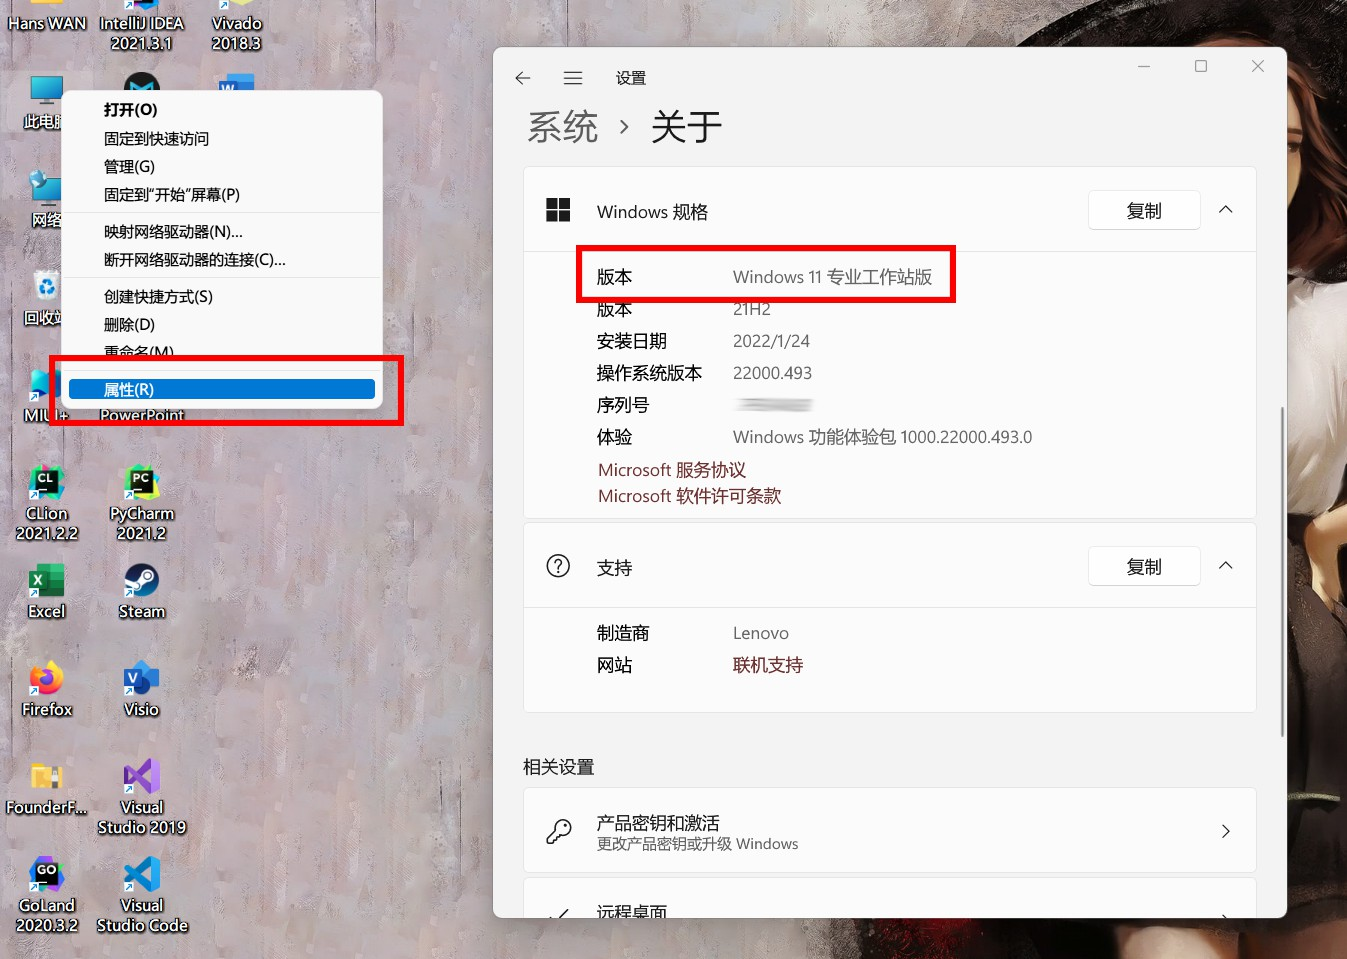
\includegraphics[width=8cm]{assets/Check_Windows_version.jpg}
  \caption{检查 Windows 系统的版本}
  \label{check-windows-version}
\end{figure}

《Missing》假定读者使用的系统是 Windows 10 或者 Windows 11,其中所有的操作都是基于 Windows 10 或者 Windows 11 简体中文版系统来描述的。如果你使用的是 Windows 7、Windows 8 或者 Windows 8.1,其中大多数操作也都能正常使用。一些明确仅能用于 Windows 10 和 / 或 Windows 11 的操作和技巧会特别标注。

\practice

\begin{enumerate}
  \item 在之前打开的【此电脑】→【属性】,你除了能看到自己电脑的 Windows 版本之外,也能找到自己电脑的处理器型号和内存容量信息。尝试去查找这个信息,并自行上网搜索你的处理器型号,辨认它的品牌、系列,判断它是几核处理器,「主频」有多高。(「主频」是描述 CPU 性能的一个指标。)
  \item 你使用的是游戏本还是轻薄本?亦或是介于二者之间的所谓「全能本」?尝试翻到笔记本的底面,上网搜索它底面所写的型号,了解关于你自己机器的更多信息。
  \item 在 Windows 10 / 11 中,打开【任务管理器】,切换到【性能】选项卡,可以看到一个更详细的硬件运行状态,其中【硬盘】相关栏目展示了你设备的硬盘数量和类型(机械硬盘 HDD、固态硬盘 SSD)。尝试查看你电脑的硬盘容量和类型。
  
  你可以通过按 \keys{Ctrl + Shift + Esc} 来打开「任务管理器」。也可以右击【开始按钮】,选择【任务管理器】来打开它。
  \begin{figure}[H]
    \centering
    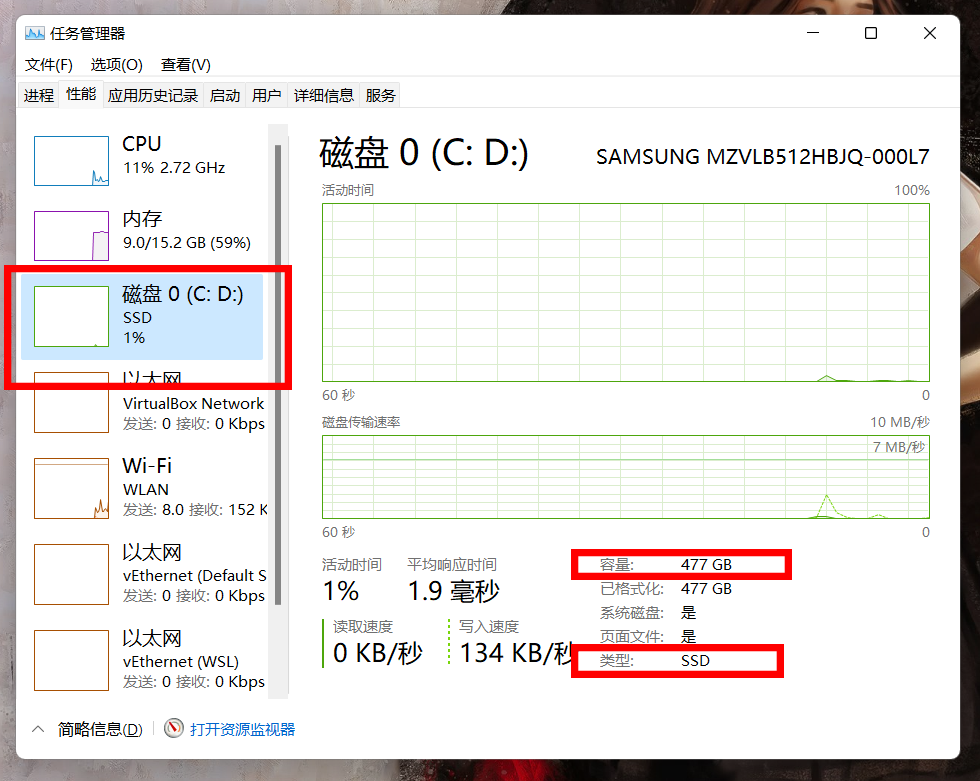
\includegraphics[width=10cm]{assets/Check_disk_status.png}
    \caption{查看电脑硬盘容量和类型}
    \label{check-disk}
  \end{figure}
  \item 你对「电路」的认知有多少?你是否好奇 CPU 是怎么运作的?从开关、导线、电池、灯泡组成的最简单「电路」到几乎无所不能「电脑」之间到底发生了什么奇妙的变化?《Missing》限于篇幅是不可能告诉你这些的。但是,你若有兴趣,可以去学习「电路电子技术」「数字电路与数字逻辑」「计算机体系结构」等相关内容。近年来,国际形势风云变幻,我国在芯片领域仍然存在许多短板。我们希望越来越多的有志青年能投身于包括但不限于体系结构、硬件组成、数字电路乃至微电子、半导体材料等领域,为我国芯片行业「补上短板」贡献自己的力量。
\end{enumerate}
